
\documentclass[ 
	% -- opções da classe memoir --
	article,			% indica que é um artigo acadêmico
	11pt,				% tamanho da fonte
	oneside,			% para impressão apenas no verso. Oposto a twoside
	a4paper,			% tamanho do papel. 
	% -- opções da classe abntex2 --
	%chapter=TITLE,		% títulos de capítulos convertidos em letras maiúsculas
	%section=TITLE,		% títulos de seções convertidos em letras maiúsculas
	%subsection=TITLE,	% títulos de subseções convertidos em letras maiúsculas
	%subsubsection=TITLE % títulos de subsubseções convertidos em letras maiúsculas
	% -- opções do pacote babel --
	english,			% idioma adicional para hifenização
	brazil,				% o último idioma é o principal do documento
	]{abntex2}


% --- 
% PACOTES
% ---

% ---
% Pacotes fundamentais 
% ---
\usepackage{cmap}				% Mapear caracteres especiais no PDF
\usepackage{lmodern}			% Usa a fonte Latin Modern
\usepackage[T1]{fontenc}		% Selecao de codigos de fonte.
\usepackage[utf8]{inputenc}		% Codificacao do documento (conversão automática dos acentos)
\usepackage{indentfirst}		% Indenta o primeiro parágrafo de cada seção.
\usepackage{nomencl} 			% Lista de simbolos
\usepackage{color}				% Controle das cores
\usepackage{graphicx}			% Inclusão de gráficos
\usepackage{csvsimple}
\usepackage{epstopdf}
%\usepackage[nolists,tablesfirst]{endfloat}
% ---
		
% ---
% Pacotes adicionais, usados apenas no âmbito do Modelo Canônico do abnteX2
% ---
\usepackage{lipsum}				% para geração de dummy text
% ---
		
% ---
% Pacotes de citações
% ---
\usepackage[brazilian,hyperpageref]{backref}	 % Paginas com as citações na bibl
\usepackage[alf]{abntex2cite}	% Citações padrão ABNT
% ---

% ---
% Configurações do pacote backref
% Usado sem a opção hyperpageref de backref
\renewcommand{\backrefpagesname}{Citado na(s) página(s):~}
% Texto padrão antes do número das páginas
\renewcommand{\backref}{}
% Define os textos da citação
\renewcommand*{\backrefalt}[4]{
	\ifcase #1 %
		Nenhuma citação no texto.%
	\or
		Citado na página #2.%
	\else
		Citado #1 vezes nas páginas #2.%
	\fi}%
% ---

% ---
% Informações de dados para CAPA e FOLHA DE ROSTO
% ---
\titulo{Relatório de atividades: Uso do classificador 1-NN, KNN e DMC na base
de dados da flor de íris} 
\autor{David Clifte\thanks{cliftedavid@gmail.com}}
\local{Brasil}
\data{2015, v-1.0}
% ---

% ---
% Configurações de aparência do PDF final

% alterando o aspecto da cor azul
\definecolor{blue}{RGB}{41,5,195}

% informações do PDF
\makeatletter
\hypersetup{
     	%pagebackref=true,
		pdftitle={\@title}, 
		pdfauthor={\@author},
    	pdfsubject={Modelo de artigo científico com abnTeX2},
	    pdfcreator={LaTeX with abnTeX2},
		pdfkeywords={abnt}{latex}{abntex}{abntex2}{atigo científico}, 
		colorlinks=true,       		% false: boxed links; true: colored links
    	linkcolor=blue,          	% color of internal links
    	citecolor=blue,        		% color of links to bibliography
    	filecolor=magenta,      		% color of file links
		urlcolor=blue,
		bookmarksdepth=4
}
\makeatother
% --- 

% ---
% compila o indice
% ---
\makeindex
% ---

% ---
% Altera as margens padrões
% ---
\setlrmarginsandblock{4cm}{4cm}{*}
\setulmarginsandblock{4cm}{4cm}{*}
\checkandfixthelayout
% ---

% --- 
% Espaçamentos entre linhas e parágrafos 
% --- 

% O tamanho do parágrafo é dado por:
\setlength{\parindent}{1.3cm}

% Controle do espaçamento entre um parágrafo e outro:
\setlength{\parskip}{0.2cm}  % tente também \onelineskip

% Espaçamento simples
\SingleSpacing

% ----
% Início do documento
% ----
\begin{document}

% Retira espaço extra obsoleto entre as frases.
\frenchspacing 

% ----------------------------------------------------------
% ELEMENTOS PRÉ-TEXTUAIS
% ----------------------------------------------------------

%---
%
% Se desejar escrever o artigo em duas colunas, descomente a linha abaixo
% e a linha com o texto ``FIM DE ARTIGO EM DUAS COLUNAS''.
% \twocolumn[    		% INICIO DE ARTIGO EM DUAS COLUNAS
%
%---
% página de titulo
\maketitle

% resumo em português
\begin{resumoumacoluna}
 Este trabalho apresentam os resultados obtidos ao aplicar os classificadores
 1-nn, KNN e DMC ao banco de dados da íris. A implementação foi feita no
 Matlab\texttrademark 
 
 
 \vspace{\onelineskip}
 
 \noindent
 \textbf{Palavras-chaves}: latex. abntex. editoração de texto.
\end{resumoumacoluna}

% ]  				% FIM DE ARTIGO EM DUAS COLUNAS
% ---

% ----------------------------------------------------------
% ELEMENTOS TEXTUAIS
% ----------------------------------------------------------
\textual

% ----------------------------------------------------------
% Introdução
% ----------------------------------------------------------
\section*{Introdução}


% ----------------------------------------------------------
% Seção de explicações
% ----------------------------------------------------------
\section{Preparação da base}
\subsection{Base de dados da flor de íris}
A base de dados da flor de íris criado por Fisher \cite{AHG2137}. Nessa base de
dados as informações obtidas das flores foram o comprimento e a largura das
pétalas e sépalas de 3 tipos de flor de íris, virgínica, versicolor e setosa.
Cada tipo de flor possue 50 instancias.

\subsection{Normalização e codificação}
\label{ss:normCodf} 
Após o carregamento da base foi realizado apenas a normalização dos dados e a
codificação dos rótulos. A normalização foi realizada separadamente para cada
atributo. Foi identificado o máximo e o mínimo do atributo $p$ e todos os
valores foram normalizados na faixa [0,1].

A codificação do rótulo foi feita no modelo 1-de-k(1-of-K ou one-hot encoding),
nesse modelo o rótulo é codificado em um vetor onde cada posição do
vetor representa uma classe. Nesse modelo para uma quantidade $m$ de classes
temos um vetor com $m$ posições e a classe $k$ é representada por um vetor
onde todas as outras posições diferentes de $k$ possuem o valor zero e a
posição $k$ possui o valor 1. Dessa forma as três classes possíveis da íris
foram codificadas em um vetor de 3 posições, onde a posição 1, 2 e 3
representam a classe setosa, versicolor e virgínica respectivamente.


%Gráfico em barra
\subsection{Análise das características}
\label{ss:analiCara}

Na figura \ref{fig:charMatrix} é apresentada a matriz de características. 
Essa matriz consiste de gráficos formados pelos pares de características
combinadas.

Na diagonal principal é apresentado o histograma do atributo.
Devido a natureza continua dos atributos do problema, pois o
comprimento e largura da sépala e pétala podem assumir qualquer valor real O
histograma foi obtido após a realização da quantização dos atributos.
Cada atributo foi quantizado em 15 possíveis valores com faixas de mesma largura. A
largura da faixa foi obtida da seguinte forma $(max_p - min_p)/15$, onde max e
min são os valores máximos e mínimos do atributo $p$.

\begin{figure}[!htb] \centering
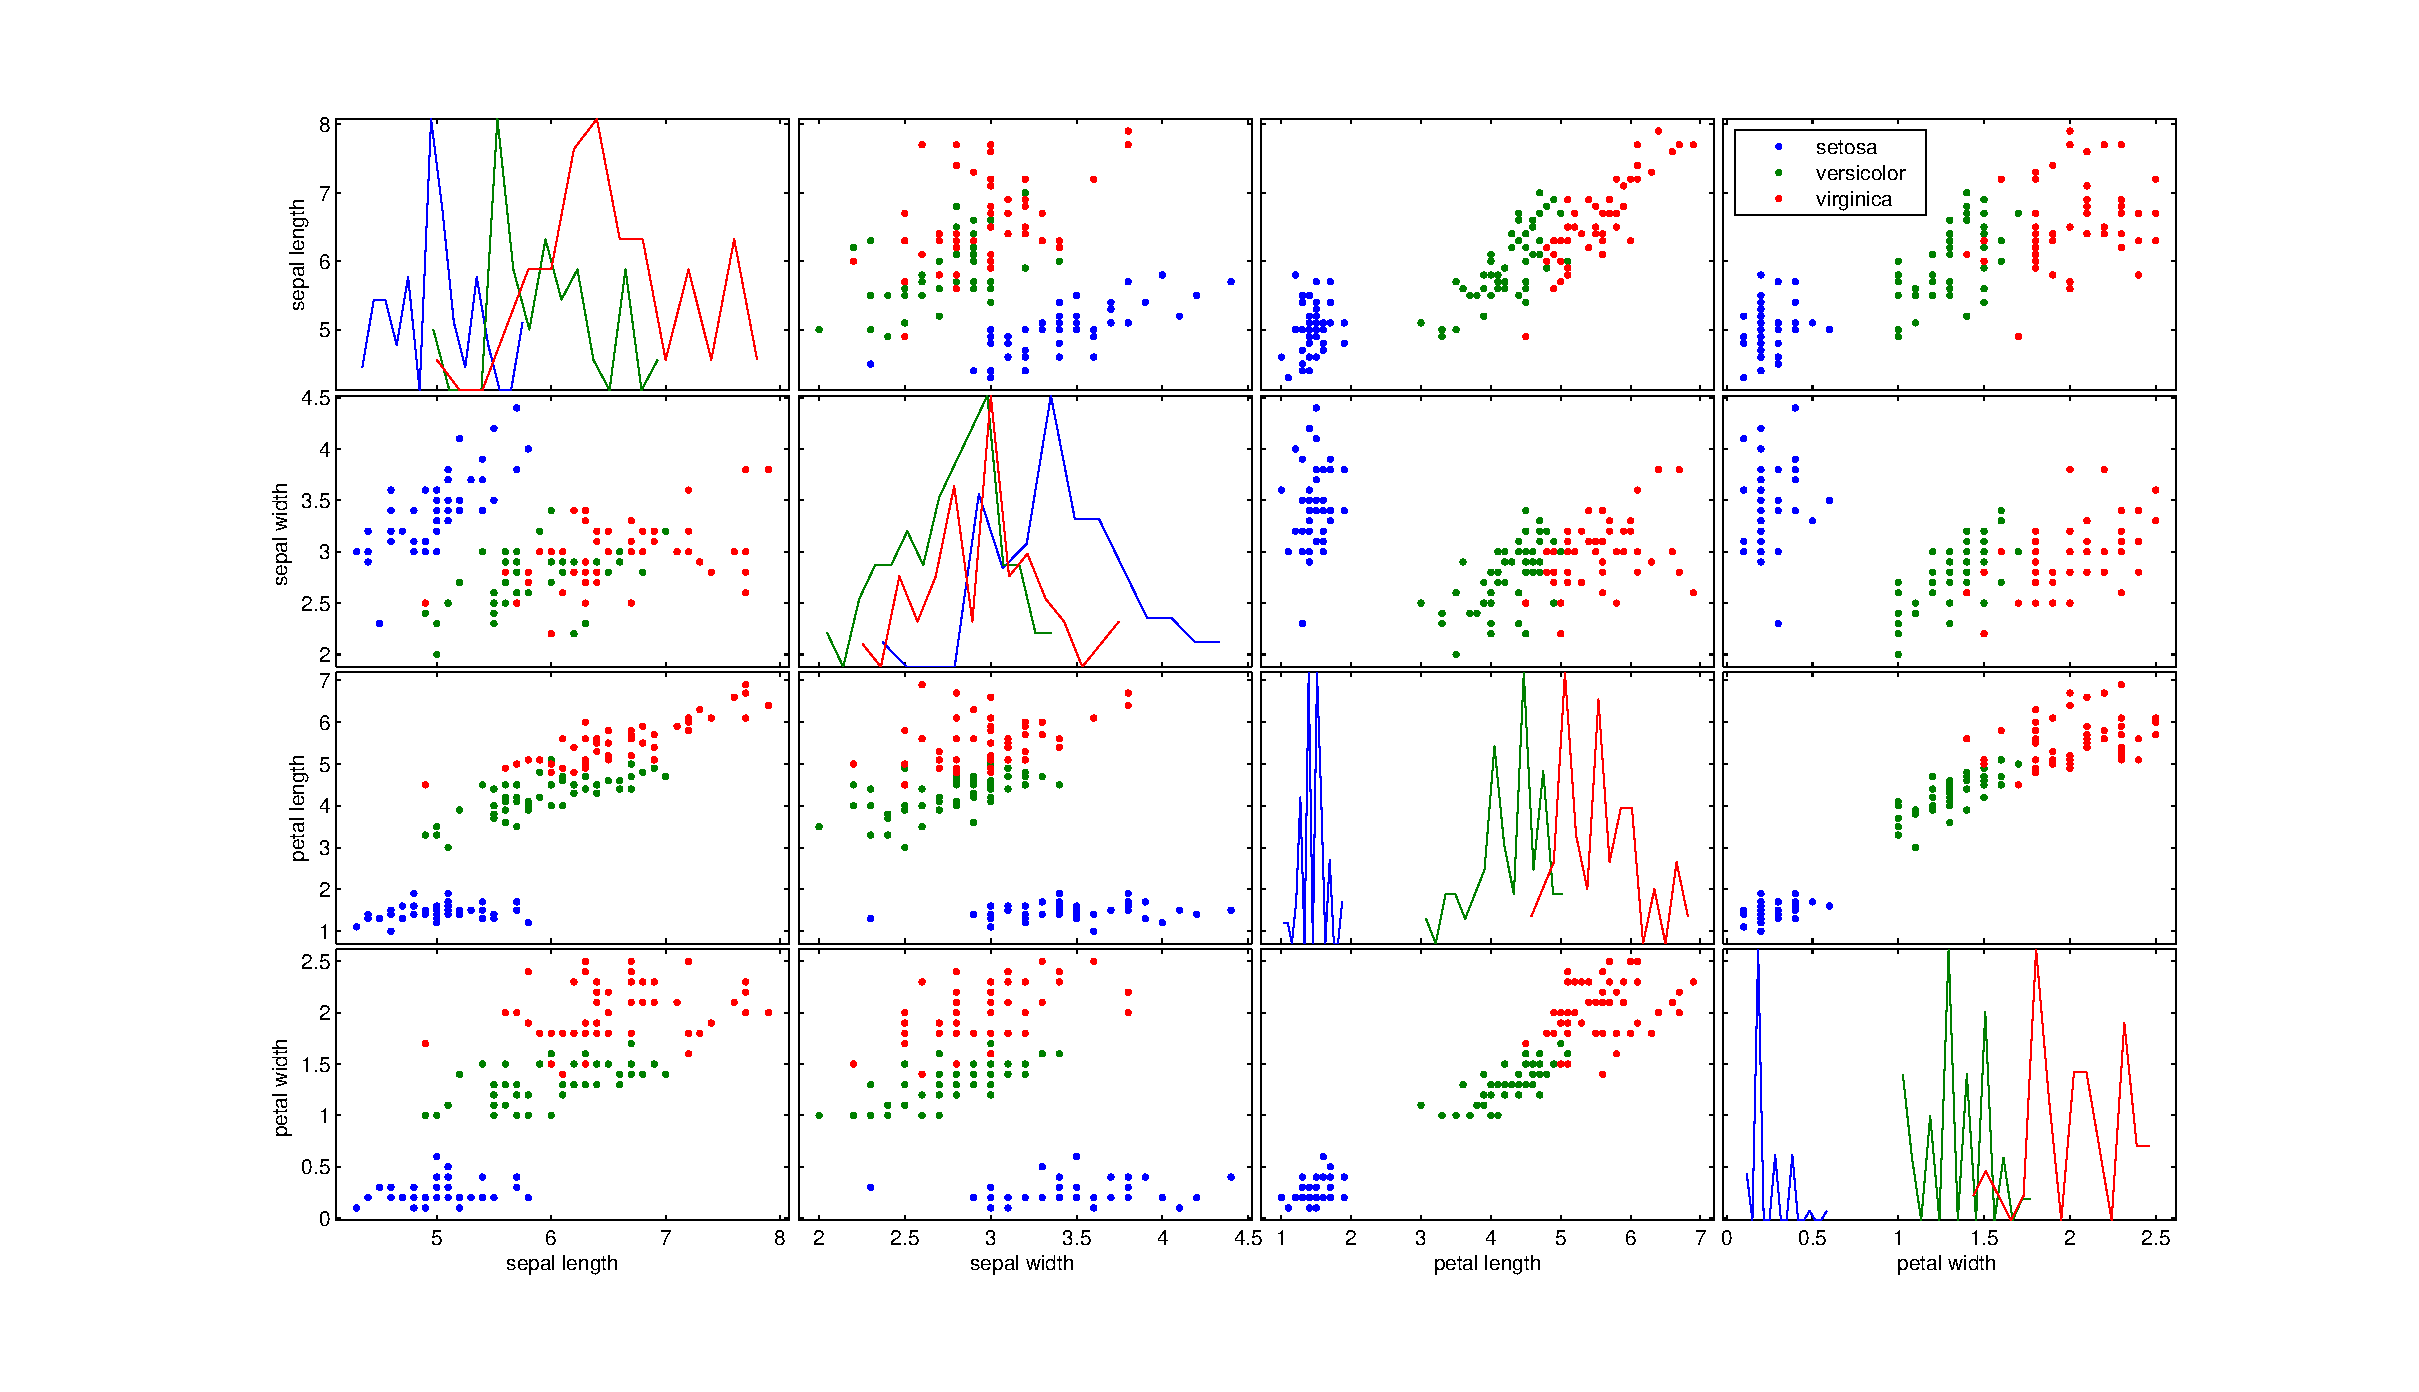
\includegraphics[width=\textwidth]{figuras/analiseIris_hist_scatterMatrix.eps}
\caption{Matriz de características.}
\label{fig:charMatrix}
\end{figure}

 Podemos perceber que a classe setosa pode facilmente ser separada das outras
 utilizando a largura ou o comprimento da pétala como variável. Nos histogramas
 localizados na parte inferior isso pode ser verificado, pétalas com
 comprimentos menores que 0,25 ou sépalas com largura menor que 0,3 de
 comprimento são claramente da classe setosa.
 Já para as duas outras características essa separação não é tão simples,
 perceba a sobreposição dos histogramas em todos os atributos bem como a mistura
 das classes nos gráficos de dispersão.
 
%\subsubsection{Análise PCA}
%  
% \subsubsection{Análise PCA}
% PCA is a standard technique for visualizing high dimensional data and for data
% pre-processing. PCA reduces the dimensionality (the number of variables) of a
% data set by maintaining as much variance as possible.
% 
% The first component, PC 1, represents the direction of the highest variance
% of the data. The direction of the second component, PC 2, represents the highest
% of the remaining variance orthogonal to the first component.
% 
%  Low variance can often be assumed to represent undesired background noise. The
% dimensionality of the data can therefore be reduced, without loss of relevant information
% 



\section{1-NN e KNN}

\subsection{Introdução}
O KNN é uma técnica que realiza a classificação de uma amotra de acordo com as k
amotras mais semelhantes existentes em sua base. Essa semelhança pode ser
quantificada atravez de uma função característica do problema ou mais comumente
atravez do calculo da distância euclidiana. O 1-NN é um caso específico do KNN
para este classificador o número de vizinhos que deve ser levado em conta é
apenas 1.

Uma importante vantagem do KNN frente ao 1-NN é a capacidade de controlar a
interferência a ruídos presentes na base de dados. Quanto maior o valor de K
mais informação será levada em consideração para a identificação da label da
amostra e considerando também que a quantidade de ruído presente próximo a
amostra é suficientemente pequena frente ao valor de K este pode ser contornado.


\subsection{Metodologia}
\label{ss:metAplKnn}

Para a avaliação do KNN foi realizado a normalização e a codificação das classe
no modelo 1-of-k, como dito na subsessão \ref{ss:normCodf}, além foi necessário
alguns outros passos para obtermos os resultados apresentados na sessão
seguinte.

Após a normalização e a codificação a base de dados foi dividida por um  de 1:4,
desta forma das 150 amostras presentes na base 30 delas foram escolhidas
aleatoriamente para pertencerem à base de testes e o restante, 120, pertencerem
a base de treinamento. É importante ressaltar também que pelo fato da escolha
dos dados de testes serem dados de forma aleatória não é possível garantir que a
base de treinamento ou teste possuem uma quantidade equivalente das 3 classes,
porém espera-se que existam aproximadamente 40 instancias de cada classe na base
de treinamento e 10 instancias de cada classe na base de teste.

Foram feitos uma série de teste variando o valor de K bem como testes de
generalização onde foi realizado a minimização da quantidade de dados
necessários na base para uma correta classificação.

\subsection{Resultados obtidos}

\subsubsection{Variação do valor de K}
Nesse teste foram realizadas 100 repetições para cada valor de K. A acurácia e o
desvio padrão são exibidos na tabela \ref{tab:acuracia}. A figura
\ref{fig:acuracia} apresenta um . 
É percebido que para o problema da íris a variação do valor de k não representa
diferença significativa para um valor de k até 30, mesmo para o valor de k igual
a 1. Para valores de K superiores a 30 podemos notar uma redução da acurácia e a
partir de 70 a média começa a dimunuir. Na faixa [60 a 110] a acurácia variou
entre 20\% e 90\% o que indica baixíssima confiabilidade no classificador. A
partir de 120 o classificar indica apenas a classe majoritária presente na base
de dados, indistintamente da amostra apresentada. No algoritmo implementado,
para valores de k acima da quantidade de dados na base o valor de k será
ajustado para esta quantidade.

\begin{table}
	\centering
    \begin{tabular}{c|c|c}%
    \bfseries K & \bfseries Acurácia & \bfseries Desvio Padrão% specify table
    % head 
    \csvreader[no head]{matlab/iris_KNN_acuracia.csv}{}% use head of
    % csv as column names
    {\\\hline\csvcoli&\csvcolii&\csvcoliii}% specify your coloumns here 
    \\\hline
    
    \end{tabular}
    \caption{Acurácia média e desvio padrão em função do valor de k.}
    \label{tab:acuracia}
\end{table}
 
\begin{figure}[!htb] \centering
	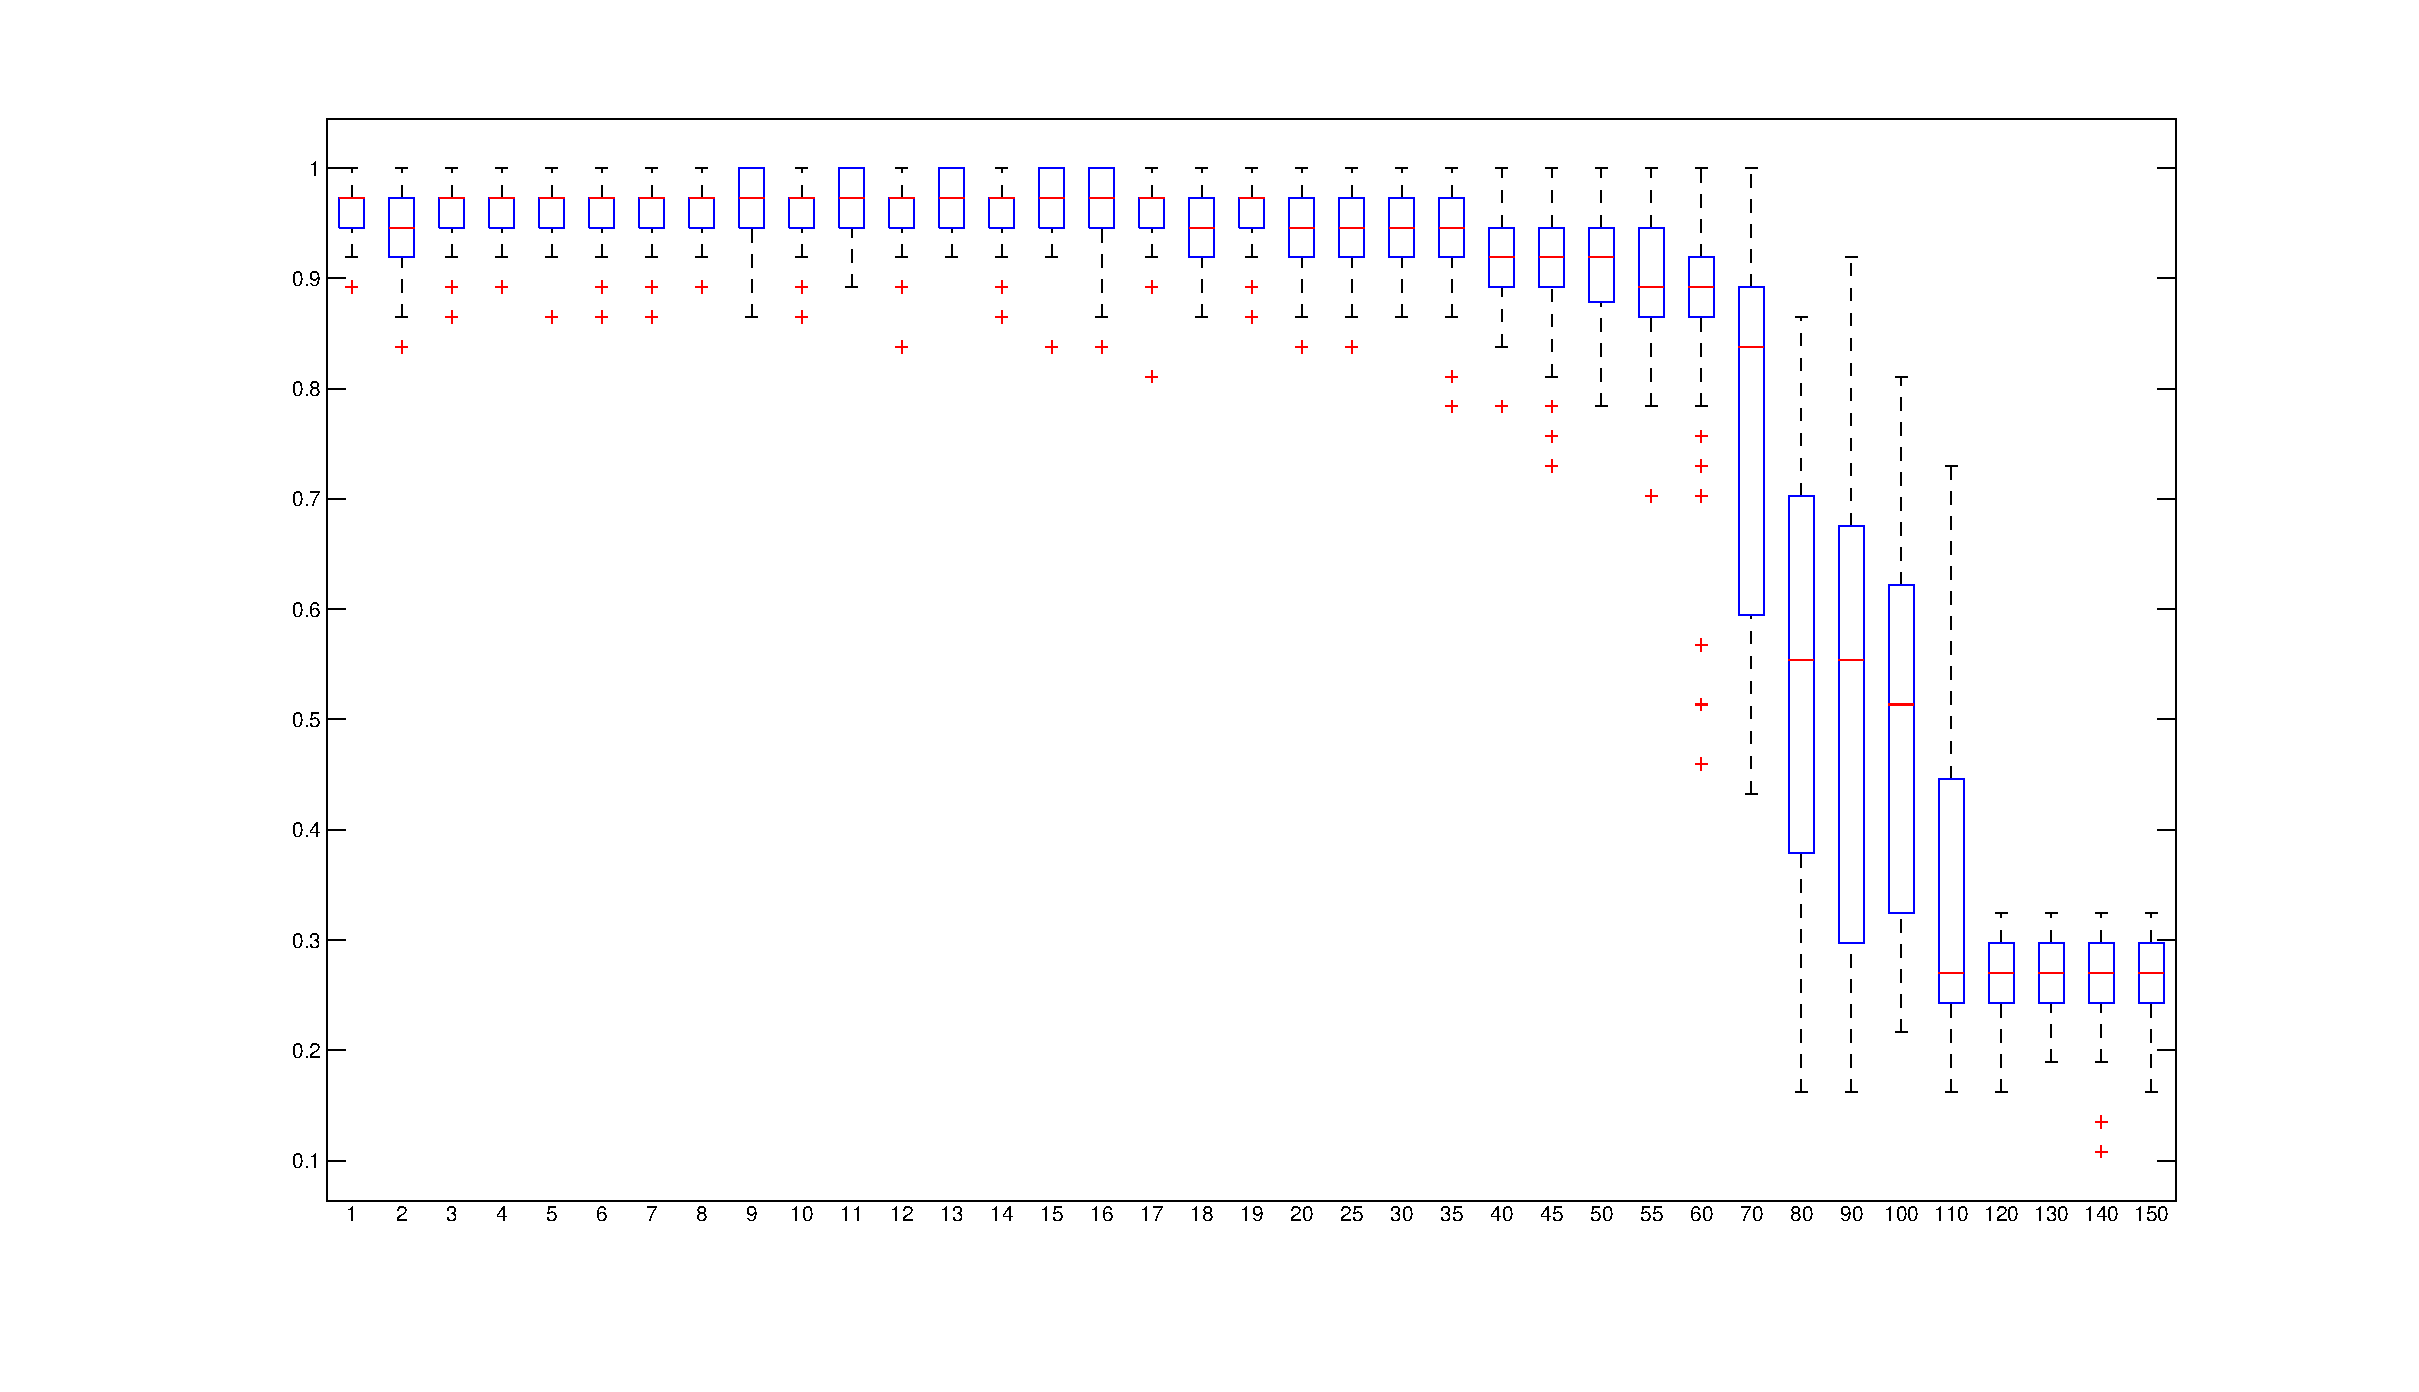
\includegraphics[width=\textwidth]{figuras/boxPlot_acuraciaVSK.eps}
	\caption{Acurácia em função do valor de k.}
	\label{fig:acuracia}
\end{figure} 


\subsubsection{Região de decisão}

Nas figuras \ref{fig:decisionRegionSepL_PetL} e
\ref{fig:decisionRegionSepL_SepW} são exibidas as regiões de decisões ao aplicar
o KNN considerando apenas duas características. Para a figura
\ref{fig:decisionRegionSepL_PetL} são consideradas apenas os atributos largura
da sépala e pétala. Um importante ponto a ser levado em consideração é que ao
descartar determinados atributos podem surgir informações duplicadas. É
importante filtrar estas informações, podem surgir linhas com informações iguais
porém rótulos diferentes o que pode causar um erro na geração região
de decisão..

Diferentes regiões de decisões foram calculadas para
diferentes valores de K. Para K=1 é notável que a existencia de ruídos podem
gerar regiões que prejudicam a generalização. Para k=5 é possível perceber que
pontos isolados não mais definem a classe de determinada região do espaço,veja
na figura \ref{fig:decisionRegionSepL_PetL} a existência de 2 pontos da classe
virgínica(em vermelho) na região em que foi classificada como da classe
versícolor(em verde). A medida que o K aumenta podemos perceber a queda no valor
da acurácia. Vários pontos são classificados de forma errada.

O mesmo se aplica para a figura \ref{fig:decisionRegionSepL_SepW}, porém nesta
foram consideradas apenas as larguras e comprimentos da sépala.


\begin{figure}
	\centering
	\begin{tabular}{cc}
	  \includegraphics[width=70mm]{matlab/figura/iris_KNN_RegDec_K1_1_3.eps} &
	  \includegraphics[width=70mm]{matlab/figura/iris_KNN_RegDec_K10_1_3.eps}
	  \\
	(a) k=1 & (b) k=10 \\[6pt] 
	 \includegraphics[width=70mm]{matlab/figura/iris_KNN_RegDec_K50_1_3.eps} &  
	 \includegraphics[width=70mm]{matlab/figura/iris_KNN_RegDec_K75_1_3.eps} \\
	(c) k=50 & (d) k=75 \\[6pt] 

	\end{tabular}

	\caption{Região de decisão utilizando Largura da sépala e da pétala.}
	\label{fig:decisionRegionSepL_PetL}
\end{figure}

\begin{figure}
	\centering
	\begin{tabular}{cc}
	  \includegraphics[width=70mm]{matlab/figura/iris_KNN_RegDec_K1_1_2.eps} &
	  \includegraphics[width=70mm]{matlab/figura/iris_KNN_RegDec_K10_1_2.eps}
	  \\
	(a) k=1 & (b) k=10 \\[6pt] 
	 \includegraphics[width=70mm]{matlab/figura/iris_KNN_RegDec_K50_1_2.eps} &  
	 \includegraphics[width=70mm]{matlab/figura/iris_KNN_RegDec_K75_1_2.eps} \\
	(c) k=50 & (d) k=75 \\[6pt] 

	\end{tabular}
	\caption{Região de decisão utilizando comprimento e largura da sépala.}
	\label{fig:decisionRegionSepL_SepW}
\end{figure}
 


\subsubsection{Matriz Confusão}
Na tabela \ref{tab:confMatKNN} é exibida a matriz confusão obtida para K igual a
10. Esse valor de k foi escolhido devido aos testes de acurácia em
função de k mostrarem que com este valor é obtida a melhor acurácia. Além da
matriz confusão  a tabela \ref{tab:knnAnalis} traz os
resultados, falso-positivo, falso-negativo, verdadeiro-positivo e
verdadeiro-negativo. 

 
\begin{table}
	\centering 
	
	\begin{tabular}{c|c}
 
	    \begin{tabular}{c}% 
	    \bfseries Classe \\\hline 
	    Setosa \\\hline
	    Versicolor \\\hline
	    Virgínica \\\hline

	    \end{tabular}   
	 
		&
	   \begin{tabular}{c|c|c|c}%
	    \bfseries Setosa & \bfseries Versicolor & \bfseries Virgínica
	    % specify table head 
	    \csvreader[no head]{matlab/iris_KNN_cmNorm.csv}{}% use head of
	    % csv as column names
	    {\\\hline\csvcoli&\csvcolii&\csvcoliii}% specify your coloumns
	    % here
	    \\\hline
     
    	\end{tabular}
    
    
	\end{tabular}
    \caption{Matriz confusão obtida após execução do KNN.}
    \label{tab:confMatKNN}
\end{table}

 

\begin{table}
	\centering
	 
	\begin{tabular}{c|c}
	 
	 \centering
	    \begin{tabular}{c}%
	    \bfseries Classe \\\hline 
	    Setosa \\\hline
	    Versicolor \\\hline
	    Virgínica \\\hline

	    \end{tabular}   
	 
		&
	   \begin{tabular}{c|c|c|c}%
	    \bfseries falso-positivo & \bfseries falso-negativo 
	    & \bfseries verdadeiro-positivo & \bfseries verdadeiro-negativo
	    % specify table head 
	    \csvreader[no head]{matlab/iris_KNN_cmAnalise.csv}{}% use head of
	    % csv as column names
	    {\\\hline\csvcoli&\csvcolii&\csvcoliii&\csvcoliv}% specify your coloumns
	    % here
	    \\\hline
     
    	\end{tabular}
    
    
	\end{tabular}
    \caption{Resultado da análise do KNN.}
    \label{tab:knnAnalis}
\end{table}











\section{DMC}
\subsection{Introdução} 
O DMC é uma técnica que realiza a classificação de uma amotra de acordo com a
amostra mais semelhantes existentes em sua base. Sua implementação é semelhante
ao KNN porém seus dados de treinamento são reduzidos ao centro de massa de cada
classe(também conhecido como centróide).
Um objeto pertence a essa classe quando a distância entre ele e o centróide for menor
que todas as distâncias entre os outros centróides restantes do espaço de características.
O primeiro passo do processo de classificação por distancia mínima é o calculo
dos  vetores médios (centróides) que representam cada classe por padrões \cite{UND:DMC13}.

\subsection{Metodologia}
A metodologia seguida para o DMC é semelhante à do KNN vista
na sessão \ref{ss:metAplKnn}, obviamente diferenciado-se pela não realização
da análise da variação do valor de K.
Foram realizadas as normalizações e codificações necessárias bem como a mesma
análise das características abordada na sessão \ref{ss:analiCara}.

\subsection{Resultados obtidos}

\subsubsection{Definição do centroide}
Devido a metodologia adotada a posição do centróide varia ao longo do cálculo da
acurácia média. Na tabelas \ref{tab:centroidesM} são exibidos os
centróides médios obtidos para o cálculo do DMC.


\begin{table}
	\centering
	
	\begin{tabular}{c|c}
	 
	    \begin{tabular}{c}%
	    \bfseries Classe \\\hline 
	    Setosa \\\hline
	    Versicolor \\\hline
	    Virgínica \\\hline

	    \end{tabular}
	
		&
	
	    \begin{tabular}{c|c|c|c}%
	    \bfseries Comprimento S & \bfseries Largura S & \bfseries Comprimento P &
	    \bfseries Largura P
	    % specify table head 
	    \csvreader[no head]{matlab/iris_DMC_meanCentroid.csv}{}% use head of
	    % csv as column names
	    {\\\hline\csvcoli&\csvcolii&\csvcoliii&\csvcoliv}% specify your coloumns
	    % here
	    \\\hline
	    
	    \end{tabular}
	\end{tabular}
    \caption{Centroides médios utilizados no DMC.}
    \label{tab:centroidesM}
\end{table}

 
% 
% \begin{table}
% 	\centering
%     \begin{tabular}{c|c|c|c}%
%     \bfseries Comprimento S & \bfseries Largura S & \bfseries Comprimento P &
%     \bfseries Largura P
%     % specify table head 
%     \csvreader[no head]{matlab/iris_DMC_STDCentroid.csv}{}% use head of
%     % csv as column names
%     {\\\hline\csvcoli&\csvcolii&\csvcoliii&\csvcoliv}% specify your coloumns
%     % here
%     \\\hline
%     
%     \end{tabular}
%     \caption{Desvio Padrão dos centroides médios utilizados no DMC.}
%     \label{tab:centroidesSTD}
% \end{table}
% 

 
\subsubsection{Região de decisão}
Na figura \ref{fig:dmc_decisionRegion} são exibidas as regiões de decisão
calculadas. Os pontos pretos ao centro de cada classe são os centroides. A
figura \ref{fig:dmc_decisionRegion}a é apresentada a região de decisão para os
atributos comprimento e largura da sépala enquanto a figura
\ref{fig:dmc_decisionRegion}b os atributos considerados são largura da sépala e
largura da pétala. Diferentemente do KNN o DMC possui uma região de decisão mais
simples e por isso menos flexível à modelagens de dados mais complexas. 

\begin{figure}
	\centering
	\begin{tabular}{cc}
	  \includegraphics[width=70mm]{matlab/figura/iris_DMC_RegDec_1_2.eps} &
	  \includegraphics[width=70mm]{matlab/figura/iris_DMC_RegDec_1_3.eps}
		\\
		(a) & (b)
	\end{tabular}
	\caption{Região de decisão utilizando o DMC.}
	\label{fig:dmc_decisionRegion}
\end{figure}
 
\subsubsection{Matriz confusão}
 Na tabela \ref{tab:confMatDMC} é exibida a matriz confusão após a execução do
 DMC. A tabela \ref{tab:DMCAnalisis} traz os
resultados, falso-positivo, falso-negativo, verdadeiro-positivo e
verdadeiro-negativo.
 
\begin{table}
	\centering
	
	\begin{tabular}{c|c}
	 
	    \begin{tabular}{c}%
	    \bfseries Classe \\\hline 
	    Setosa \\\hline
	    Versicolor \\\hline
	    Virgínica \\\hline

	    \end{tabular}
	 
		&
	   \begin{tabular}{c|c|c|c}%
	    \bfseries Setosa & \bfseries Versicolor & \bfseries Virgínica
	    % specify table head 
	    \csvreader[no head]{matlab/iris_DMC_cmNorm.csv}{}% use head of
	    % csv as column names
	    {\\\hline\csvcoli&\csvcolii&\csvcoliii}% specify your coloumns
	    % here
	    \\\hline
    
    	\end{tabular}
    
    
	\end{tabular}
    \caption{Matriz confusão obtida após execução do DMC.}
    \label{tab:confMatDMC}
\end{table}
 
 
 
 
\begin{table}
	\centering
	
	\begin{tabular}{c|c}
	 
	    \begin{tabular}{c}%
	    \bfseries Classe \\\hline 
	    Setosa \\\hline
	    Versicolor \\\hline
	    Virgínica \\\hline

	    \end{tabular}   
	 
		&
	   \begin{tabular}{c|c|c|c}%
	    \bfseries falso-positivo & \bfseries falso-negativo 
	    & \bfseries verdadeiro-positivo & \bfseries verdadeiro-negativo
	    % specify table head 
	    \csvreader[no head]{matlab/iris_KNN_cmAnalise.csv}{}% use head of
	    % csv as column names
	    {\\\hline\csvcoli&\csvcolii&\csvcoliii&\csvcoliv}% specify your coloumns
	    % here
	    \\\hline
     
    	\end{tabular}
    
    
	\end{tabular}
    \caption{Resultado da análise do KNN.}
    \label{tab:DMCAnalisis}
\end{table}


 
 
 
\bookmarksetup{startatroot}% 
% ---

% ---
% Conclusão
% ---
\section*{Considerações finais}
Podemos concluir que o KNN,  indiferentemente da forma como os dados estão
dispostos no espaço, é possível separar as regiões por mais irregulares que
sejam. O KNN possui um parâmetro que permite regular a confiabilidade de
determinado ponto no espaço, reduzindo assim a incidencia de ruídos.

Apesar de não ser apresentado nenhuma avaliação de desempenho neste relatório, é
notável a diferença entre os tempos de execução de ambas as técnicas.
 



\addcontentsline{toc}{section}{Considerações finais}



% ----------------------------------------------------------
% ELEMENTOS PÓS-TEXTUAIS
% ----------------------------------------------------------
\postextual

% ----------------------------------------------------------
% Referências bibliográficas
% ----------------------------------------------------------
\bibliography{abntex2-modelo-references,iris}

% ----------------------------------------------------------
% Glossário
% ------------------------------------ ----------------------
%
% Há diversas soluções prontas para glossário em LaTeX. 
% Consulte o manual do abnTeX2 para obter sugestões.
% 
%\glossary 

% ----------------------------------------------------------
% Apêndices
% ----------------------------------------------------------


\end{document}